%%
%% Automatically generated file from DocOnce source
%% (https://github.com/hplgit/doconce/)
%%
%%
% #ifdef PTEX2TEX_EXPLANATION
%%
%% The file follows the ptex2tex extended LaTeX format, see
%% ptex2tex: https://code.google.com/p/ptex2tex/
%%
%% Run
%%      ptex2tex myfile
%% or
%%      doconce ptex2tex myfile
%%
%% to turn myfile.p.tex into an ordinary LaTeX file myfile.tex.
%% (The ptex2tex program: https://code.google.com/p/ptex2tex)
%% Many preprocess options can be added to ptex2tex or doconce ptex2tex
%%
%%      ptex2tex -DMINTED myfile
%%      doconce ptex2tex myfile envir=minted
%%
%% ptex2tex will typeset code environments according to a global or local
%% .ptex2tex.cfg configure file. doconce ptex2tex will typeset code
%% according to options on the command line (just type doconce ptex2tex to
%% see examples). If doconce ptex2tex has envir=minted, it enables the
%% minted style without needing -DMINTED.
% #endif

% #define PREAMBLE

% #ifdef PREAMBLE
%-------------------- begin preamble ----------------------

\documentclass[%
oneside,                 % oneside: electronic viewing, twoside: printing
final,                   % draft: marks overfull hboxes, figures with paths
10pt]{article}

\listfiles               %  print all files needed to compile this document

\usepackage{relsize,makeidx,color,setspace,amsmath,amsfonts,amssymb}
\usepackage[table]{xcolor}
\usepackage{bm,ltablex,microtype}

\usepackage[pdftex]{graphicx}

\usepackage[T1]{fontenc}
%\usepackage[latin1]{inputenc}
\usepackage{ucs}
\usepackage[utf8x]{inputenc}

\usepackage{lmodern}         % Latin Modern fonts derived from Computer Modern

% Hyperlinks in PDF:
\definecolor{linkcolor}{rgb}{0,0,0.4}
\usepackage{hyperref}
\hypersetup{
    breaklinks=true,
    colorlinks=true,
    linkcolor=linkcolor,
    urlcolor=linkcolor,
    citecolor=black,
    filecolor=black,
    %filecolor=blue,
    pdfmenubar=true,
    pdftoolbar=true,
    bookmarksdepth=3   % Uncomment (and tweak) for PDF bookmarks with more levels than the TOC
    }
%\hyperbaseurl{}   % hyperlinks are relative to this root

\setcounter{tocdepth}{2}  % levels in table of contents

% Tricks for having figures close to where they are defined:
% 1. define less restrictive rules for where to put figures
\setcounter{topnumber}{2}
\setcounter{bottomnumber}{2}
\setcounter{totalnumber}{4}
\renewcommand{\topfraction}{0.95}
\renewcommand{\bottomfraction}{0.95}
\renewcommand{\textfraction}{0}
\renewcommand{\floatpagefraction}{0.75}
% floatpagefraction must always be less than topfraction!
% 2. ensure all figures are flushed before next section
\usepackage[section]{placeins}
% 3. enable begin{figure}[H] (often leads to ugly pagebreaks)
%\usepackage{float}\restylefloat{figure}

% prevent orhpans and widows
\clubpenalty = 10000
\widowpenalty = 10000

% --- end of standard preamble for documents ---


% insert custom LaTeX commands...

\raggedbottom
\makeindex
\usepackage[totoc]{idxlayout}   % for index in the toc
\usepackage[nottoc]{tocbibind}  % for references/bibliography in the toc

%-------------------- end preamble ----------------------

\begin{document}

% matching end for #ifdef PREAMBLE
% #endif

\newcommand{\exercisesection}[1]{\subsection*{#1}}


% ------------------- main content ----------------------



% ----------------- title -------------------------

\thispagestyle{empty}

\begin{center}
{\LARGE\bf
\begin{spacing}{1.25}
PHY321: Classical Mechanics 1
\end{spacing}
}
\end{center}

% ----------------- author(s) -------------------------

\begin{center}
{\bf Homework 10, due Friday  April 26${}^{}$} \\ [0mm]
\end{center}

\begin{center}
% List of all institutions:
\end{center}
    
% ----------------- end author(s) -------------------------

% --- begin date ---
\begin{center}
Apr 16, 2021
\end{center}
% --- end date ---

\vspace{1cm}


\paragraph{Practicalities about  homeworks and projects.}
\begin{enumerate}
\item You can work in groups (optimal groups are often 2-3 people) or by yourself. If you work as a group you can hand in one answer only if you wish. \textbf{Remember to write your name(s)}!

\item Homeworks are available  the week before the deadline. 

\item How do I(we)  hand in?  Due to the corona virus and many of you not being on campus, we recommend that you scan your handwritten notes and upload them to D2L. If you are ok with typing mathematical formulae using say Latex, you can hand in everything as a single jupyter notebook at D2L. The numerical exercise(s) should always be handed in as a jupyter notebook by the deadline at D2L. 
\end{enumerate}

\noindent
\paragraph{Introduction to homework 10.}
This homework is optional but gives an extra score of 10\% on top of
all you have done throughout the semester. The exercises are
essentially good old fashioned paper and pencil exercises and each
covers different aspects of what has been done after spring break.
The relevant reading background is marked in the different exercises (Taylor's text).

\paragraph{Exercise 1 (10pt), new reference frame (Taylor chapter 8).}
Show that if one transforms to a reference frame where the total
momentum is zero, $\bm{p}_1=-\bm{p}_2$, that the relative momentum
$\bm{q}$ corresponds to either $\bm{p}_1$ or $-\bm{p}_2$. This
means that in this frame the magnitude of $\bm{q}$ is one half the
magnitude of $\bm{p}_1-\bm{p}_2$.

\paragraph{Exercise 2 (10pt) Center of mass and relative coordinates (Taylor chapter 8).}
Given the center of mass and relative coordinates $\bm{R}$ and $\bm{r}$, respectively, for
particles of mass $m_1$ and $m_2$, find the coordinates $\bm{r}_1$
and $\bm{r}_2$ in terms of the masses, $\bm{R}$ and $\bm{r}$.


\paragraph{Exercise 3 (30pt),  Two-body problems (Taylor chapter 8).}
Consider a particle of mass $m$ moving in a potential
\[
V(r)=\alpha\ln(r/\alpha),
\]
where $\alpha$ is a constant.

\begin{itemize}
\item 3a (5pt)  If the particle is moving in a circular orbit of radius $R$, find the angular frequency $\dot{\theta}$. Solve this by setting $F=-m\dot{\theta}^2r$ (force and acceleration point inward).

\item 3b (5pt) Express the angular momentum $L$ in terms of the constant $\alpha$, the mass $m$ and the radius $R$. Also express $R$ in terms of $L$, $\alpha$ and $m$.

\item 3c (5pt) Sketch the effective radial potential, $V_{\rm eff}(r)$, for a particle with angular momentum $L$. (No longer necessarily moving in a circular orbit.)

\item 3d (5pt)  Find the position of the minimum of $V_{\rm eff}$ in terms of $L$, $\alpha$ and $m$, then compare to the result of (3b).

\item 3e (5pt)  What is the effective spring constant for a particle at the minimum of $V_{\rm eff}$? Express your answer in terms of $L$, $m$ and $\alpha$. 

\item 3f (5pt)  What is the angular frequency, $\omega$, for small oscillations of $r$ about the $R_{\rm min}$?  Express your answer in terms of $\dot{\theta}$ from part (3a).
\end{itemize}

\noindent
\paragraph{Exercise 4 (10pt), Lagrangian formalism (Taylor chapters 6-7).}
Consider a mass $m$ connected to a spring with spring constant $k$. Rather than being fixed, the other end of the spring oscillates with frequency $\omega$ and amplitude $A$. For a generalized coordinate, use the displacement of the mass from its relaxed position and call it $y=x-\ell-A\cos\omega t$. In this system the potential energy of the spring is $ky^2/2$.

\begin{itemize}
\item 4a (5pt) Write the kinetic energy in terms of the generalized coordinate

\item 4b (5pt) Write down the Lagrangian and find the equations of motion for $y$
\end{itemize}

\noindent
\paragraph{Exercise 5 (40pt), Pendulum and Lagrangians (Taylor chapters 6-7).}
A mathematical pendulum consists of a point mass $m$ suspended by a massless thread/rod of length $l$ in a gravitational field, as shown in the figure here. The constraining force is labeled by $\bm{T}$
and the gravitational force is labeled $\bm{F}_g$.



\vspace{6mm}

% inline figure
\centerline{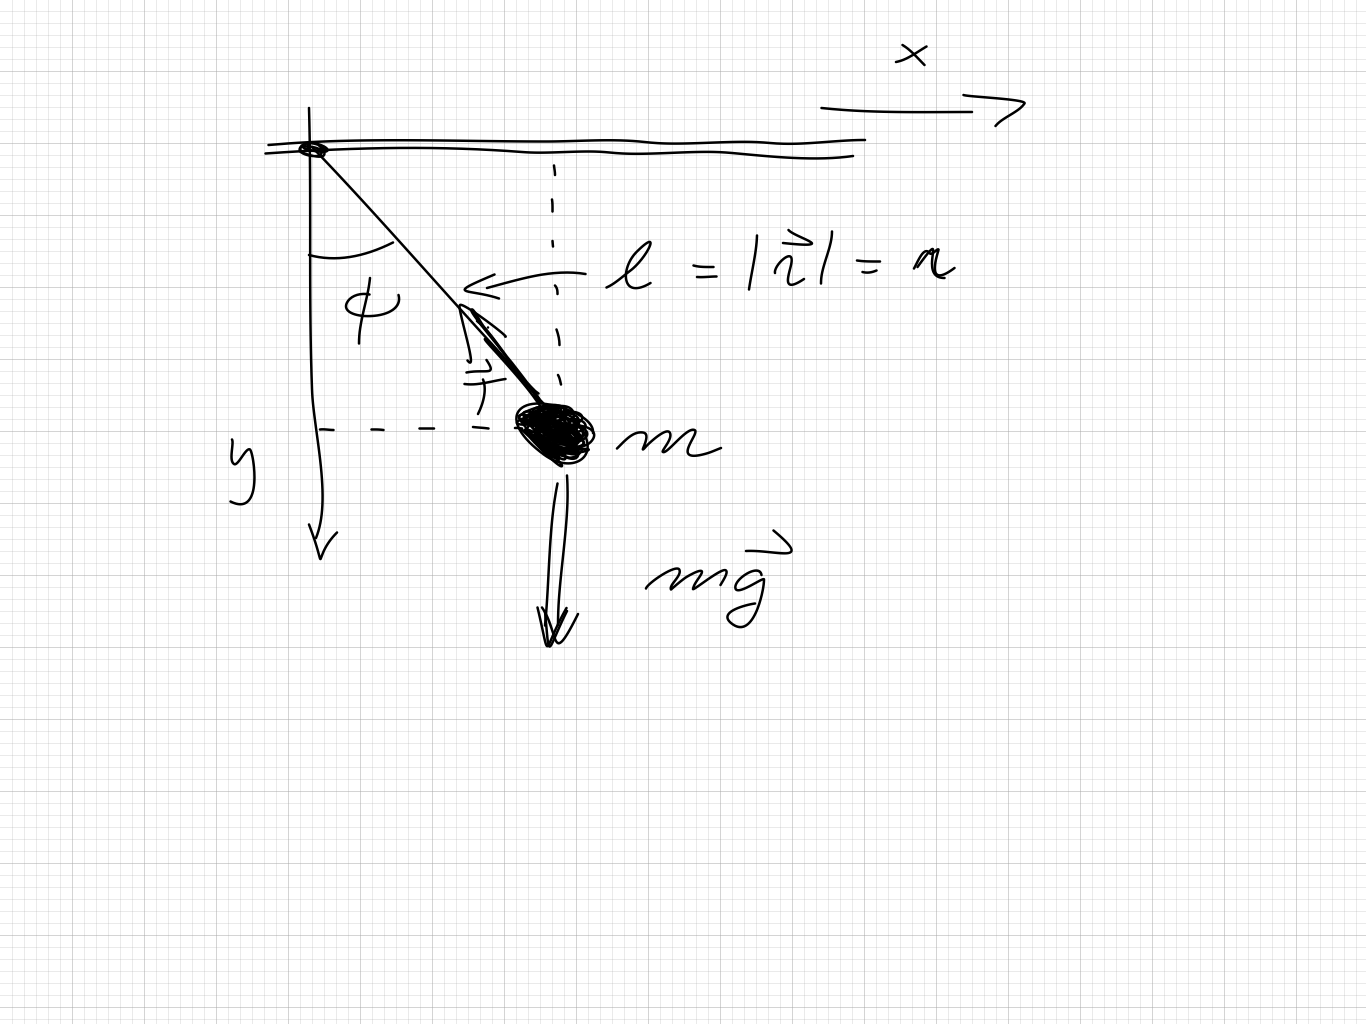
\includegraphics[width=0.6\linewidth]{figures/Simplependulum.png}}

\vspace{6mm}



We assume that the length $l$ is constant and we define the coordinates involved as

\[
\bm{r} = l\sin(\phi)\bm{\hat{x}}+l\cos(\phi)\bm{\hat{y}},
\]
where $\bm{\hat{x}}$ and $\bm{\hat{y}}$ are the unit vectors in the $x$ and $y$ directions, respectively.

\begin{itemize}
\item \textbf{5a (10pt):} Set up the forces acting on the system and show that the equation of motion is $m\ddot{\bm{r}}=\bm{F}_g+\bm{T}$.

\item \textbf{5b (10pt):} Show that you can rewrite the above equation of motion as two independent equations of motion, one for $\phi$ and one for the constraining force. Show that these equations are $\ddot{\phi}(t)=-\omega_0^2\sin{(\phi(t))}$ with $\omega_0^2=g/l$ and $T=ml\dot{\phi}^2+mg\cos{(\phi)}$.
\end{itemize}

\noindent
The equation for $\phi$ is a second-order differential equation
\[
\ddot{\phi}(t)=-\omega_0^2\sin{(\phi(t))}.
\]

This equation can be solved analytically if we assume that the angle $\phi$ is very small. Then we can approximate our equation as

\[
\ddot{\phi}(t)=-\omega_0^2\phi(t).
\]

\begin{itemize}
\item \textbf{5c (5pt):} Find the analytical solution for the last equation. Hint, look back at the solutions for the simple harmonic oscillator problem in one dimension in for example homework 7.

\item \textbf{5d (5pt):} Find the expressions for the kinetic and potential energies in terms of the variables $r$ and $\phi$. 

\item \textbf{5e (10pt):} With the potential $V$  and kinetic $T$ energies, define the Lagrangian for the mathematical pendulum discussed here. Add the constraint $r=l$ via a Lagrange multiplier $\lambda$ and derive the equations of motion. Show that these result in  $\ddot{\phi}(t)=-\omega_0^2\sin{(\phi(t))}$ with $\omega_0^2=g/l$ and $\lambda=ml\dot{\phi}^2+mg\cos{(\phi)}$.  How would you interpret $\lambda$? 
\end{itemize}

\noindent
\paragraph{Classical Mechanics Extra Credit Assignment: Scientific Writing and attending Talks.}
The following gives you an opportunity to earn \textbf{five extra credit
points} on each of the remaining homeworks and \textbf{ten extra credit points}
on the midterms and finals.  This assignment also covers an aspect of
the scientific process that is not taught in most undergraduate
programs: scientific writing.  Writing scientific reports is how
scientist communicate their results to the rest of the field.  Knowing
how to assemble a well written scientific report will greatly benefit
you in you upper level classes, in graduate school, and in the work
place.

The full information on extra credits is found at \href{{https://github.com/mhjensen/Physics321/blob/master/doc/Homeworks/ExtraCredits/}}{\nolinkurl{https://github.com/mhjensen/Physics321/blob/master/doc/Homeworks/ExtraCredits/}}. There you will also find examples on how to write a scientific article. 
Below you can also find a description on how to gain extra credits by attending scientific talks.


This assignment allows you to gain extra credit points by practicing
your scientific writing.  For each of the remaining homeworks you can
submit the specified section of a scientific report (written about the
numerical aspect of the homework) for five extra credit points on the
assignment.  For the two midterms and the final, submitting a full
scientific report covering the numerical analysis problem will be
worth ten extra points.  For credit the grader must be able to tell
that you put effort into the assignment (i.e.~well written, well
formatted, etc.).  If you are unfamiliar with writing scientific
reports, \href{{https://github.com/mhjensen/Physics321/blob/master/doc/Homeworks/ExtraCredits/IntroductionScientificWriting.md}}{see the information here}

The following table explains what aspect of a scientific report is due
with which homework.  You can submit the assignment in any format you
like, in the same document as your homework, or in a different one.
Remember to cite any external references you use and include a
reference list.  There are no length requirements, but make sure what
you turn in is complete and through.  If you have any questions,
please contact Julie Butler at butler@frib.msu.edu.


\begin{quote}
\begin{tabular}{ccc}
\hline
\multicolumn{1}{c}{ HW/Project } & \multicolumn{1}{c}{ Due Date } & \multicolumn{1}{c}{ Extra Credit Assignment } \\
\hline
HW 3               & 2-8           & Abstract                   \\
HW 4               & 2-15          & Introduction               \\
HW 5               & 2-22          & Methods                    \\
HW 6               & 3-1           & Results and Discussion     \\
\textbf{Midterm 1} & \textbf{3-12} & \emph{Full Written Report} \\
HW 7               & 3-22          & Abstract                   \\
HW 8               & 3-29          & Introduction               \\
HW 9               & 4-5           & Results and Discussion     \\
\textbf{Midterm 2} & \textbf{4-16} & \emph{Full Written Report} \\
HW 10              & 4-26          & Abstract                   \\
\textbf{Final}     & \textbf{4-30} & \emph{Full Written Report} \\
\hline
\end{tabular}
\end{quote}

\noindent

You can also gain extra credits if you attend scientific talks.
This is described here.


\paragraph{Integrating Classwork With Research.}
This opportunity will allow you to earn up to 5 extra credit points on a Homework per week. These points can push you above 100\% or help make up for missed exercises.
In order to earn all points you must:

\begin{enumerate}
\item Attend an MSU research talk (recommended research oriented Clubs is  provided below)

\item Summarize the talk using at least 150 words

\item Turn in the summary along with your Homework.
\end{enumerate}

\noindent
Approved talks:
Talks given by researchers through the following clubs:
\begin{itemize}
\item Research and Idea Sharing Enterprise (RAISE)​: Meets Wednesday Nights Society for Physics Students (SPS)​: Meets Monday Nights

\item Astronomy Club​: Meets Monday Nights

\item Facility For Rare Isotope Beam (FRIB) Seminars: ​Occur multiple times a week
\end{itemize}

\noindent
If you have any questions please consult Jeremy Rebenstock, rebensto@msu.edu.

All the material on extra credits is at \href{{https://github.com/mhjensen/Physics321/blob/master/doc/Homeworks/ExtraCredits/}}{\nolinkurl{https://github.com/mhjensen/Physics321/blob/master/doc/Homeworks/ExtraCredits/}}. 












% ------------------- end of main content ---------------

% #ifdef PREAMBLE
\end{document}
% #endif

